\documentclass[10pt]{article}

\usepackage[margin=0.9in]{geometry}
\usepackage{graphicx}
\usepackage{amsmath}
\usepackage{amssymb}
\usepackage{booktabs}
\usepackage{caption}
\usepackage{hyperref}
\usepackage{enumitem}
\usepackage{titlesec}
\usepackage{parskip}

\hypersetup{
    colorlinks=true,
    linkcolor=blue,
    citecolor=blue,
    urlcolor=blue
}

% Tight section spacing
\titlespacing*{\section}{0pt}{6pt}{2pt}
\titlespacing*{\subsection}{0pt}{4pt}{1pt}
\titleformat{\section}{\normalfont\large\bfseries}{\thesection}{0.5em}{}
\titleformat{\subsection}{\normalfont\normalsize\bfseries}{\thesubsection}{0.5em}{}

% Tight float spacing
\setlength{\textfloatsep}{6pt plus 1pt minus 1pt}
\setlength{\floatsep}{6pt plus 1pt minus 1pt}
\setlength{\intextsep}{6pt plus 1pt minus 1pt}
\setlength{\abovecaptionskip}{2pt}
\setlength{\belowcaptionskip}{0pt}

% Tight list spacing
\setlist{topsep=2pt,itemsep=1pt,parsep=0pt}

% Paragraph spacing
\setlength{\parskip}{6pt plus 2pt minus 1pt}
\setlength{\parindent}{0pt}

\title{\vspace{-2em}From Spikes to Scenes: Neural Image Reconstruction from Marmoset Visual Cortex in the Data-Limited Regime\vspace{-0.5em}}
\author{Jared Yao, Spring 2026}
\date{\vspace{-2em}}

\begin{document}

\maketitle

\section{Introduction}

The primate ventral visual stream builds a rich, tolerant representation that supports robust and invariant object recognition, and a compelling test of how well we understand this representation is whether we can reconstruct the perceived image directly from neural activity. Recent work has achieved this by aligning brain responses to the latent spaces of diffusion models, from fMRI (Takagi and Nishimoto, 2023; Scotti et al., 2024) and more recently from intracortical spiking activity in macaque (Ciferri et al., 2026). Crucially, all prior approaches rely on large datasets (22{,}000+ images or thousands of trials) atypical of most primate neurophysiology. Whether reconstruction is feasible in the data-limited regime (a few hundred stimuli, invasive electrophysiology) remains open.

We address this using Neuropixels 1.0 recordings from marmoset ventral stream cortices during passive viewing of the HVM dataset (DiCarlo et al., 2012) with 450 images spanning 10 categories $\times$ 45 variations. Key challenges include severe data scarcity (80$\times$ fewer training pairs than MindEye2), noisy pseudo-population responses pooled across sessions, the need to separate object-level from scene-level signals, and limited spatial control in the generative model.

\section{Methods}

\subsection{Neural Encoder}

We train two lightweight MultiHeadTransformer encoders (Figure~\ref{fig:encoder}), each predicting an L2-normalised SigLIP-SO400M (1152-d) and category CLIP (768-d) embedding from the neural response. The global model targets the full-image SigLIP, while the object model targets SigLIP of the GDINO-cropped object region. This separation is neurobiologically motivated, because the ventral stream encodes a position- and size-invariant representation that aligns more closely with the object crop than with the full image. Both encoders share the same architecture, with a learned category embedding added to the shared latent as a low-data inductive bias. The shared latent doubles as an interpretable probe of the neural population, providing a compressed summary of ventral stream representations that can be analyzed independently of generation.

The training loss combines per-head InfoNCE and cosine regression with a uniformity penalty on the shared latent:
\begin{equation}
\mathcal{L} = w_{\text{sig}} \Bigl[\alpha\,\mathcal{L}^{\text{sig}}_{\text{NCE}} + (1-\alpha)\,\mathcal{L}^{\text{sig}}_{\text{cos}}\Bigr] + w_{\text{clip}} \Bigl[\alpha\,\mathcal{L}^{\text{clip}}_{\text{NCE}} + (1-\alpha)\,\mathcal{L}^{\text{clip}}_{\text{cos}}\Bigr] + w_{\text{unif}}\,\mathcal{L}_{\text{unif}}
\end{equation}
where $\alpha$ controls the InfoNCE/cosine tradeoff and $\mathcal{L}_{\text{unif}}$ penalises collapsed shared latents. The best configuration used is \texttt{d\_model=64}, \texttt{n\_heads=4}, \texttt{n\_layers=2}, \texttt{shared\_dim=512}.

\begin{figure}[h]
    \centering
    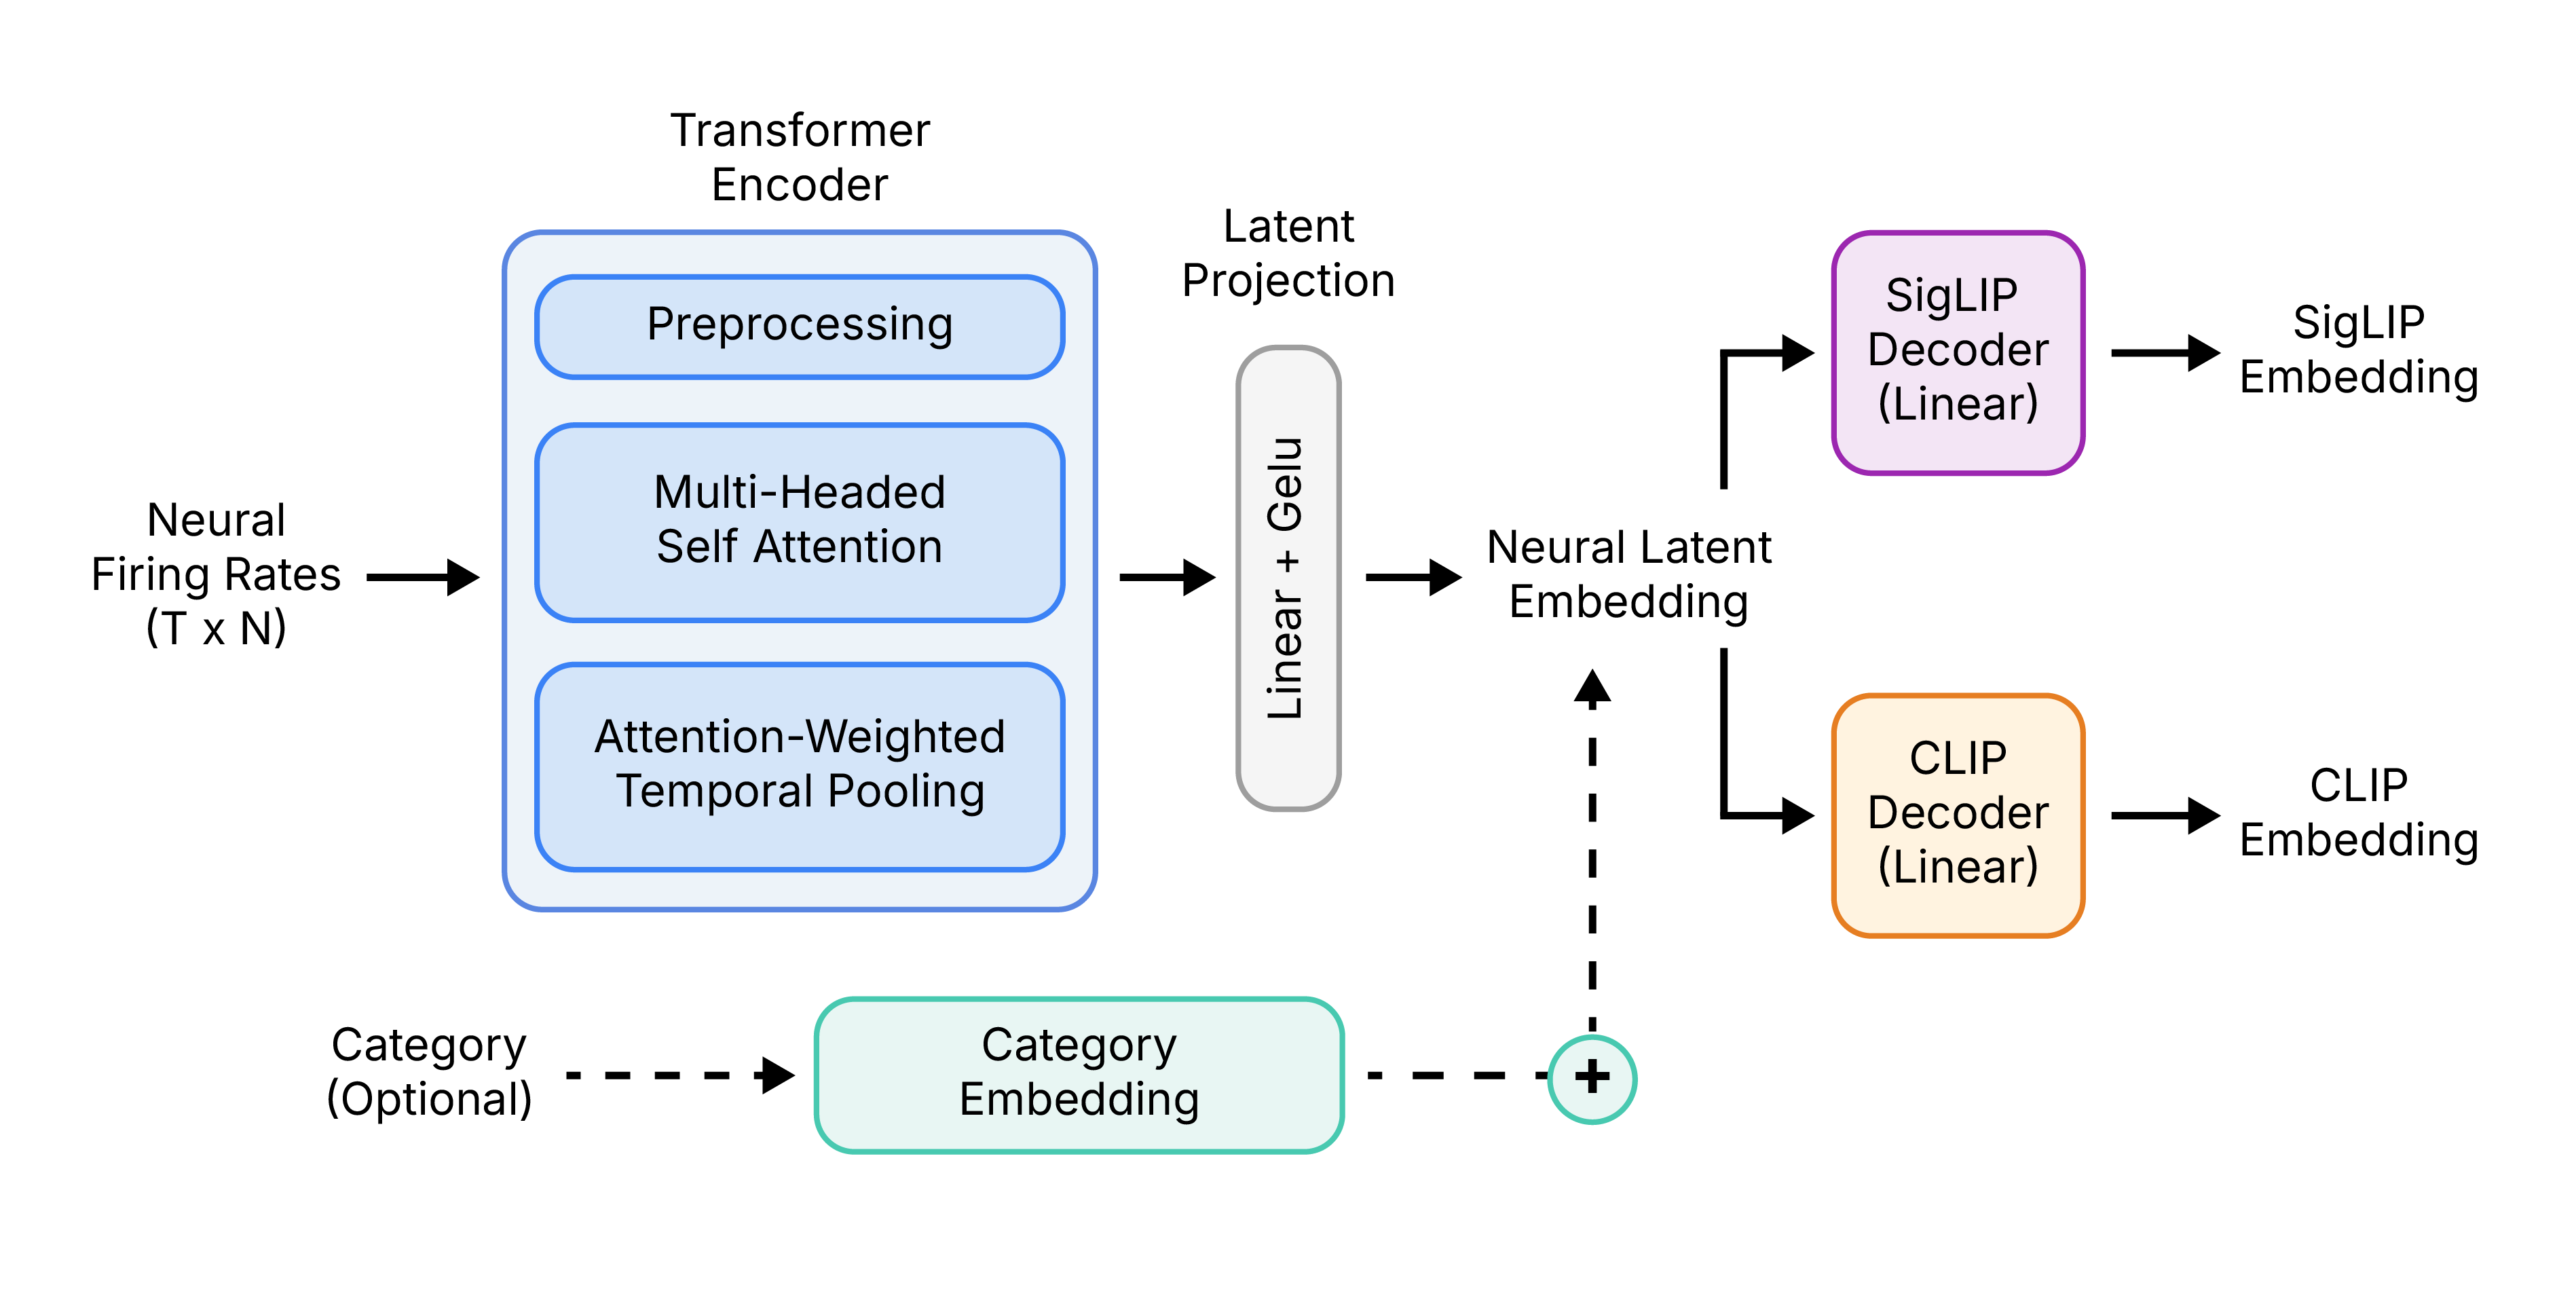
\includegraphics[width=0.6\linewidth]{figures/encoder diagram.png}
    \caption{MultiHeadTransformer architecture.}
    \label{fig:encoder}
\end{figure}

\subsection{Conditioned Generation}

Predicted embeddings condition a pretrained FLUX.1-dev via the pretrained InstantX/FLUX.1-dev-IP-Adapter with no finetuning. Generation uses a sequential two-pass img2img procedure (Figure~\ref{fig:pipeline}), in which each pass starts from the source image noised to a fixed strength (controlling how much of the input is preserved versus regenerated) and runs the corresponding fraction of denoising steps:
\begin{enumerate}[leftmargin=*]
    \item Pass 1 (object recovery). The GDINO bbox crop is denoised conditioned on $z_{\text{sig\_obj}}$, then composited back onto the original to form a spliced latent.
    \item Pass 2 (global recovery). Starts from the original init latent conditioned on $z_{\text{sig\_global}}$. At each step, bbox tokens are blended toward the spliced latent with a cosine-decaying weight (0.6 to 0), anchoring object structure early and releasing it late. Latents outside the circular aperture are pinned to the original.
\end{enumerate}

Four conditions are evaluated: Control, Text-only (category name), Neural pred (predicted embeddings), and GT upper bound (ground-truth embeddings).

\begin{figure}[h]
    \centering
    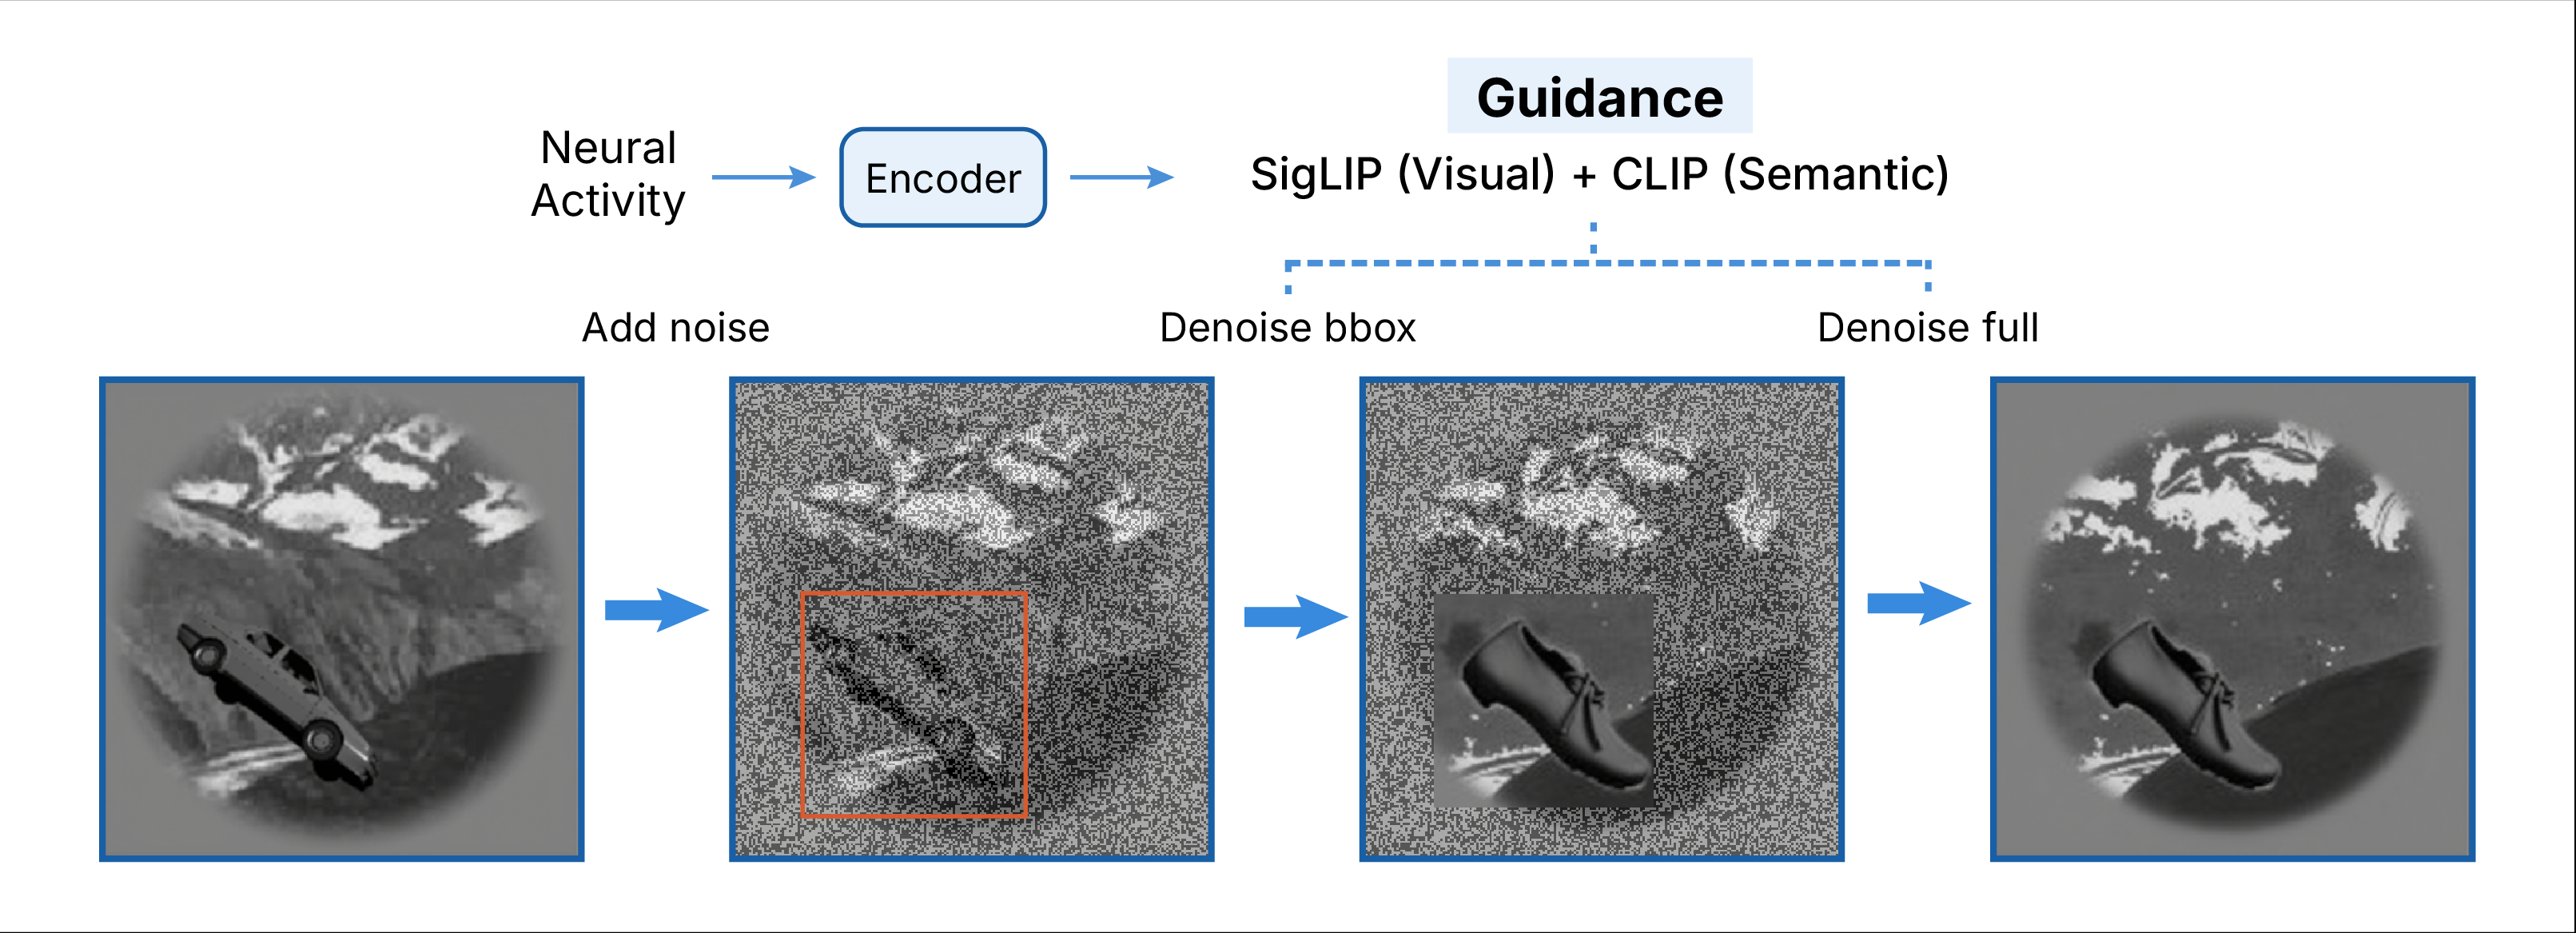
\includegraphics[width=\linewidth]{figures/pipeline horizontal.png}
    \caption{Two-pass generation pipeline. Neural activity is encoded to SigLIP (visual) and CLIP (semantic) guidance. Pass 1 denoises the GDINO bounding-box crop, and the result is composited back before Pass 2 denoises the full image, producing the final reconstruction within the circular aperture.}
    \label{fig:pipeline}
\end{figure}

\section{Results}

\subsection{Encoder Generalization}

Both models generalize to held-out test stimuli, confirming that 270 training examples are sufficient to recover stimulus-specific embedding information from noisy pseudo-population neural responses. Above-chance 2-AFC accuracy on both heads indicates that predicted embeddings are measurably closer to the correct ground-truth than to the 89 distractors.

\begin{table}[h]
    \centering\small
    \begin{tabular}{lcccc}
        \toprule
        Model & SigLIP cos sim & CLIP cos sim & SigLIP 2-AFC & CLIP 2-AFC \\
        \midrule
        Global model & 0.8331 & 0.9834 & 0.9663 & 0.9101 \\
        Object model & 0.8804 & 0.9886 & 0.9582 & 0.9101 \\
        \bottomrule
    \end{tabular}
    \caption{Embedding cosine similarity and 2-AFC identification accuracy (chance = 0.5) on the 90 test stimuli.}
    \label{tab:encoder}
\end{table}

\subsection{Neural Pred Matches or Exceeds Text-Guided Reconstruction Quality}

Across the 90 test stimuli, neural pred reconstructions are visually comparable to or better than text-conditioned reconstructions, despite the text condition receiving the ground-truth category label through both T5 and CLIP pooled embeddings. Since the high-dimensional T5 embeddings provide rich semantic information that the neural pathway lacks, the encoder must recover the semantic content from a small, noisy pseudo-population. That neural pred remains competitive indicates that the recovered embeddings carry sufficient signal to drive the generative model, even in the low training data regime.

\subsection{Decoding Object Gesture}

The most diagnostic stimuli are those in which object pose, viewpoint, or spatial configuration vary substantially within a category. As shown in Figure~\ref{fig:results}A (bottom rows), neural pred reconstructions recover these within-category variations in several examples, producing outputs whose object gesture and surface texture align with the original stimulus more closely than those of the text condition, which is blind to pose and can misplace the foreground object onto background elements of the scene. This is direct evidence that the encoder captures stimulus-specific visual structure beyond category membership.

\subsection{Failure Cases Reveal the Limits of the Ventral Population Representation}

The gap between neural pred and GT-guided reconstructions is itself informative. Because GT supplies the ground-truth embeddings, any quality that GT recovers but neural pred does not reflects information present in the stimulus image yet absent from the predicted neural embeddings, offering a direct readout of what the marmoset ventral population fails to encode reliably.

Two patterns stand out in Figure~\ref{fig:results}B. On the face stimuli, GT-guided reconstruction recovers fine facial details while neural pred produces a face-shaped object without recognizable features, likely due to the marmoset's failure of face identification in this specific stimulus. On the elephant stimuli, both text-guided and GT-guided reconstructions recover plausible elephants, whereas neural pred consistently struggles to reconstruct the elephant, suggesting a general difficulty of the population signal in encoding this category.

\begin{figure}[t]
    \centering
    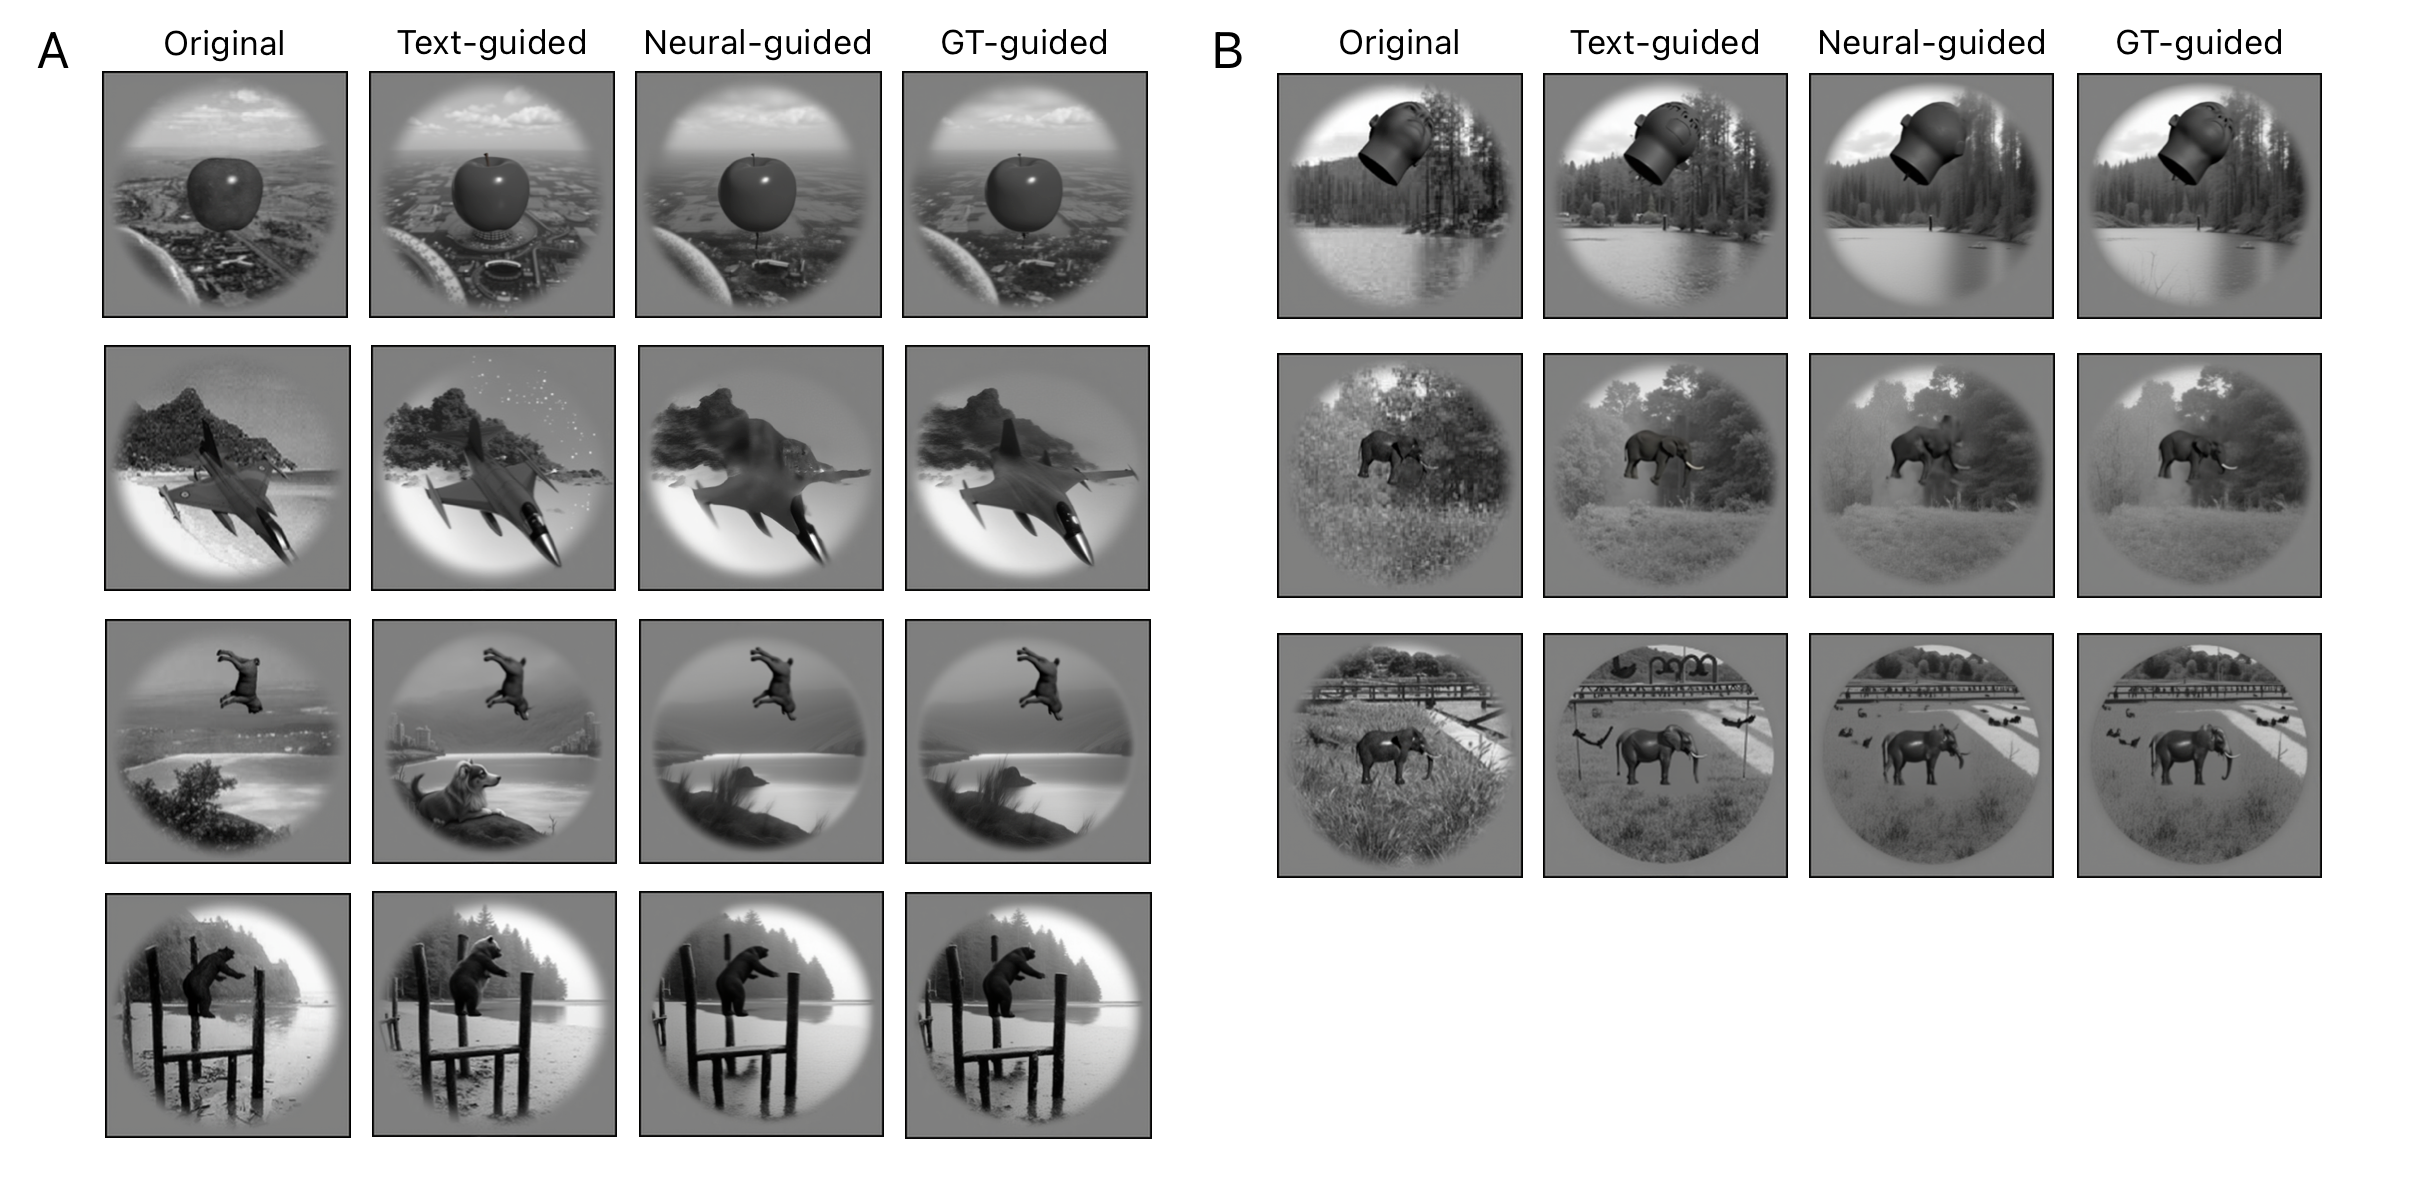
\includegraphics[width=\linewidth]{figures/figure3.png}
    \caption{Four-column composite strips (Original $\mid$ Text-guided $\mid$ Neural-guided $\mid$ GT-guided) for representative test stimuli. \textbf{(A)} Neural-guided reconstruction recovers within-category gesture and viewpoint that the text condition cannot. \textbf{(B)} Failure cases: neural pred produces face-shaped objects without recognizable features and fails to recover elephant shape, while text-guided and GT-guided reconstructions succeed.}
    \label{fig:results}
\end{figure}

\section{Discussion}

The results demonstrate that neural image reconstruction is feasible in the data-limited regime typical of primate electrophysiology. A lightweight encoder trained on only 270 examples generalizes to held-out stimuli, and the resulting reconstructions match or exceed those produced from the ground-truth category label. The ability to decode within-category object gesture, including pose, viewpoint, and spatial configuration that are invisible to the text condition, indicates that the ventral population signal carries fine-grained visual structure beyond category membership, while the two-pass pipeline supports this by aligning Pass 1 with the ventral stream's position- and size-invariant object code and using the cosine-decaying bbox blend in Pass 2 to recover global coherence without hard boundary artifacts. Failure cases are equally informative. The gap between neural pred and the GT upper bound localizes what the ventral population fails to encode, providing a tool for probing the content encoded in the marmoset ventral representation.

Several directions would strengthen these conclusions. First, the current evaluation reports only embedding-space metrics; adding pixel and perceptual measures (e.g.\ SSIM) inside the HVM aperture would quantify how much pixel-level fidelity neural conditioning adds beyond the img2img baseline and how close it comes to the original stimulus. Second, the IP-Adapter is used frozen and relies on generalization from its natural-photograph training distribution to HVM stimuli, so a lightweight LoRA finetune of the adapter's key/value projections on the 270 HVM training images would test whether domain adaptation closes the remaining gap to the original stimulus.

\section*{References}
\addcontentsline{toc}{section}{References}

\small
\begin{itemize}[leftmargin=*,topsep=0pt,itemsep=0pt]
    \item J.\ J.\ DiCarlo, D.\ Zoccolan, and N.\ C.\ Rust. How does the brain solve visual object recognition? \textit{Neuron}, 73(3):415--434, 2012.
    \item Y.\ Takagi and S.\ Nishimoto. High-resolution image reconstruction with latent diffusion models from human brain activity. \textit{CVPR}, 2023.
    \item P.\ Scotti et al. MindEye2: Shared-subject models enable fMRI-to-image with 1 hour of data. \textit{arXiv:2403.11207}, 2024.
    \item M.\ Ciferri, M.\ Ferrante, and N.\ Toschi. Simple models, rich representations: Visual decoding from primate intracortical neural signals. \textit{arXiv:2601.11108}, 2026.
    \item H.\ Ye et al. IP-Adapter: Text compatible image prompt adapter for text-to-image diffusion models. \textit{arXiv:2308.06721}, 2023.
\end{itemize}

\end{document}
